\documentclass[12pt]{article}
\textwidth 15.5cm \oddsidemargin 0cm \topmargin -1cm \textheight
24cm \footskip 1.5cm \usepackage{epsfig}
\usepackage{amsmath,graphicx,psfrag,pstcol}
\def\n{\noindent}
\def\u{\underline}
\def\hs{\hspace}
\newcommand{\thrfor}{.^{\displaystyle .} .}
\newcommand{\bvec}[1]{{\bf #1}}

\begin{document}

\noindent
\rule{15.7cm}{0.5mm}


\begin{center}
{\bf ENGINEERING TRIPOS PART II A}
\end{center}
\vspace{0.5cm} {\bf EIETL \hfill MODULE EXPERIMENT 3F3}
\vspace{0.5cm}
\begin{center}
{\bf RANDOM VARIABLES and RANDOM NUMBER GENERATION\\
Short  Report \\\hfill \\Name: Harry Sarson \\\hfill\\
College: Pembroke \\\hfill
\\
Date: 03/11/2017
}
\end{center}
\rule{15.7cm}{0.5mm}



\vspace*{1cm}
\vspace*{1cm}

\begin{enumerate}
\item {\bf Uniform and normal random variables.}

Histogram of Gaussian random numbers overlaid on exact Gaussian curve (scaled):
 

\begin{figure}
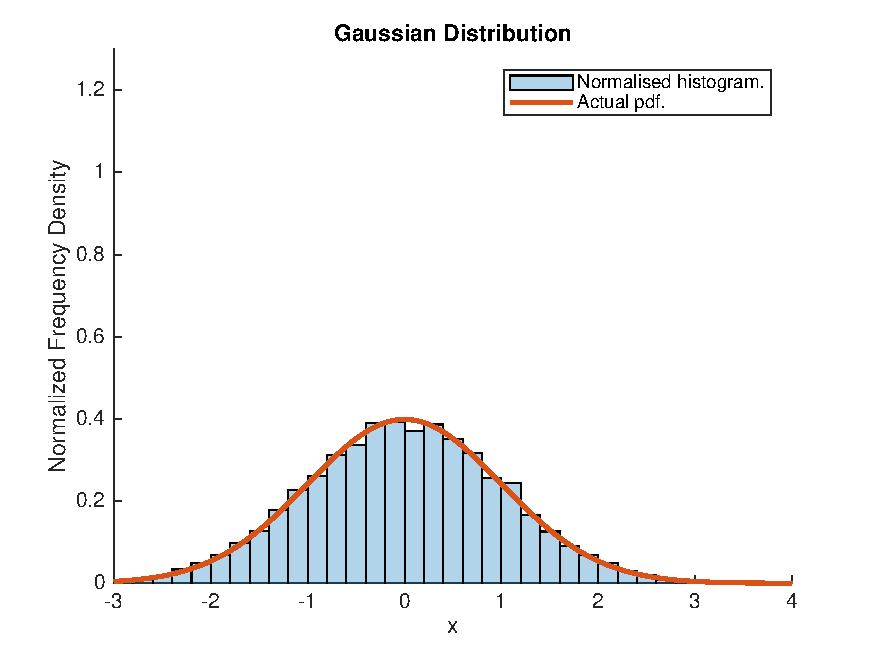
\includegraphics[width=\textwidth]{figures/gaussian-histogram.pdf}
  \caption{Histogrammed samples taken from a Gaussian distrubution.}
\end{figure}

{\em Include your graphic here}
\vspace{3in}



Kernel density estimate for Gaussian random numbers overlaid on exact Gaussian curve:


{\em Include your graphic here}
\vspace{3in}



Kernel density estimate for Uniform random numbers overlaid on exact Gaussian curve:


{\em Include your graphic here}
\vspace{3in}

Comment on the advantages and disadvantages of the kernel density method compared with the histogram method for estimation of a probability density from random samples:


{\em Text answer  here}
\vspace{3in}



Theoretical  mean and standard deviation calculation for uniform density as a function of $N$:


{\em Text/maths answer  here}
\vspace{3in}


Explain behaviour as $N$ becomes large:

{\em Text/maths answer  here}
\vspace{3in}



Plot of histograms for $N=100$,  $N=1000$ and $N=10000$ with theoretical mean  and $\pm 3$ standard deviation lines:


{\em Include your graphic here}
\vspace{3in}




 Are your histogram results consistent with the multinomial distribution theory? 


{\em Text/maths answer  here}
\vspace{3in}


\item {\bf Functions of random variables}
For normally distributed ${\cal N}(x|0,1)$ random variables, take $y=f(x)=ax+b$. Calculate $p(y)$ using the Jacobian formula:


{\em Text/maths answer  here}
\vspace{3in}


Explain how this is linked to the general normal density with non-zero mean and non-unity variance:


{\em Text/maths answer  here}
\vspace{3in}



 Verify this formula by transforming a large collection of random samples $x^{(i)}$ to give $y^{(i)}=f(x^{(i)})$, histogramming the resulting $y$ samples, and overlaying a plot of your formula calculated using the Jacobian:


{\em Include your graphic here}
\vspace{3in}




Now take $p(x)={\cal N}(x|0,1)$ and $f(x)=x^2$. Calculate $p(y)$ using the Jacobian formula:

{\em Text/maths answer  here}
\vspace{3in}




 Verify your result by histogramming of transformed random samples:


{\em Include your graphic here}
\vspace{3in}


\item{\bf Inverse CDF method} 



Calculate the CDF and the inverse CDF for the exponential distribution: 


{\em Text/maths answer  here}
\vspace{3in}



Matlab code for inverse CDF method for generating samples from the exponential distribution:


{\em Matlab code  here}
\vspace{3in}



Plot histograms/ kernel density estimates and overlay them on the desired exponential density:


{\em Include your graphic here}
\vspace{3in}

\item {\bf Simulation from a `difficult'  density.}

Matlab code to generate $N$ random numbers drawn from the distribution of $X$:
\vspace{3in}

Plot some histogram density estimates with $\alpha=0.5,\,1.5$ and several values of $\beta$:

\vspace{3in}


Hence comment on the interpretation of the parameters $\alpha$ and $\beta\in[-1,+1]$:


\end{enumerate}



\end{document}



\end{document}


